\chapter{Conception et choix technologiques}

\section*{Introduction}
Dans le cycle de vie d'un projet, l'achèvement de la phase d'analyse et de spécification des besoins aboutit à la phase de conception. Cette dernière représente la base du développement du projet. Elle définira la manière dont les besoins et les objectifs précédemment évoqués seront réalisés. Dans ce chapitre, nous allons commencer par présenter les intérêts d’UML en indiquant l’outil de conception choisi. Ensuite, nous allons étudier la modélisation et la représentation de la vue dynamique en utilisant les diagrammes de séquences et celle de la vue statique en utilisant le diagramme de classes.

\section{Intérêts d’UML}
    Unified Modeling Language (UML) est un langage de modélisation unifié qui permet de modéliser les solutions apportées aux problèmes avec des notations unifiées comme les diagrammes. Un des tous premiers avantages d'UML, est de favoriser la communication entre les utilisateurs et les informaticiens.

UML est un outil incontournable de modélisation. Il s’approprié une approche de développement incrémentale et itérative \cite{UML}.

   \section{L’outil de conception : PowerAMC} 
   L’outil «PowerAMC» offre plusieurs méthodes de modélisation, accessibles aux informaticiens de tout niveau, parmi elles : Merise, UML, Data Warehouse, et processus métiers\cite{PowerAmc}.\\
   Cet outil est retenu pour la représentation des schémas des différents diagrammes (d’utilisation, de classes et de séquences).
   
        
       \section{Diagramme de classes} 
       Le diagramme de classes est une représentation statique des éléments qui constituent l'application.. Il représente les classes participantes dans l'application\cite{DiagrammeClasse}.
       La figure \ref{fig:Diagramme de classes} ci-dessous expose les différentes classes qui existent dans l’application.
       
       \newpage
         \begin{figure}[htpb]
\centering
\fcolorbox{blue}{white}{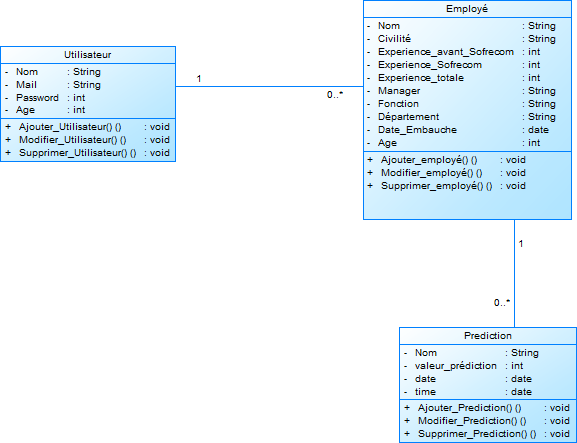
\includegraphics[width=1\linewidth]{img/DiagClasse.png}}
\caption{Diagramme de classes}
\label{fig:Diagramme de classes}
\end{figure} 
L'utilisateur contient plusieurs informations (nom, prénom,mot de passe...) et il peut gérer plusieurs employés qui sont caracterisés chacun d'entre eux par son nom,son expérience et sa date d'embauche...

Pour chaque employé, il peut avoir une ou plusieurs prédiction qui représente la démission de ce dernier.

\newpage
  \section{Diagrammes de séquences} 
  L’étude du projet est effectuée en adoptant une conception dynamique ayant pour but de donner des scénarios de déroulement des différentes tâches de l’application. Des diagrammes de séquences sont élaborés.\\
  Le diagramme de séquences correspond à des échanges des informations entre les éléments dans le cas de fonctionnement de l’application \cite{DiagSeq}.
   \subsection{Diagramme de séquences <<importer un fichier>>}
   L’utilisateur choisit d'abord un fichier d’extension ".csv". Un traitement d’appel est fait ensuite des différentes opérations (PostFile, Parse, ParseSetup et Split (0.25 , 0 .75)) de la part de notre application qui interagit avec H2o.ai. Enfin, L’utilisateur choisit le nom de modèle à construire.
La figure \ref{fig:Diagramme de séquences <<importer un fichier>>} ci-dessous décrit le déroulement du processus de la réalisation de cette tâche.
         \begin{figure}[htpb]
\centering
\fcolorbox{black}{white}{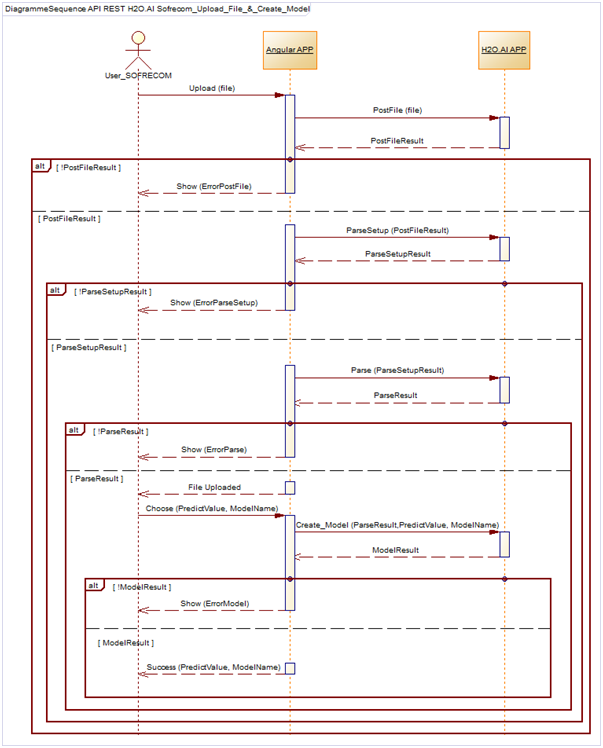
\includegraphics[width=1\linewidth]{img/diagseq1.png}}
\caption{Diagramme de séquences <<importer un fichier>>}
\label{fig:Diagramme de séquences <<importer un fichier>>}
\end{figure}
\newpage

 \subsection{Diagramme de séquences <<Effectuer une Prediction>>}
 La prédiction est la fonctionnalité la plus importante dans notre application.Pour effectuer ce traitement,l'application doit d'abord convertir les données à prédire en un fichier d'extension ".csv". Après, l'application interagit avec H2o.ai via ce fichier.\\
 Les différentes étapes de cette fonctionnalité sont représentées dans la figure ci-après.
         \begin{figure}[htpb]
\centering
\fcolorbox{black}{white}{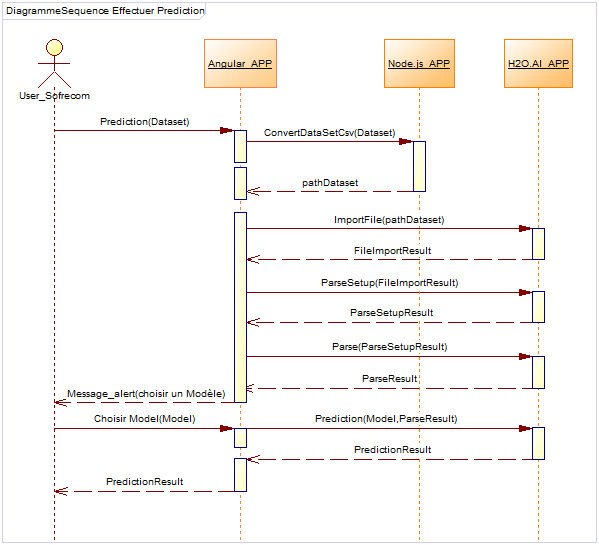
\includegraphics[width=1\linewidth]{img/diagseq2.png}}
\caption{Diagramme de séquences <<Effectuer une prédiction>>}
\label{fig:Diagramme de séquences <<Effectuer une Prediction>>}
\end{figure}

\newpage

\section*{Conclusion}
  Dans ce chapitre, nous avons présenté la conception aussi bien générale que détaillée de notre application. Le chapitre suivant, sera consacré à la partie implémentation de notre application en se basant sur la conception présentée dans ce chapitre.